% Permission is granted to copy, distribute and/or modify this document
% under the terms of the GNU Free Documentation License, Version 1.3
% or any later version published by the Free Software Foundation;
% with no Invariant Sections, no Front-Cover Texts, and no Back-Cover Texts.
% A copy of the license is included in the section entitled "GNU
% Free Documentation License".
%
% Written (C) 2012 Chiyuan Zhang

\chapter{Multiclass learning}

In this chapter we describe multiclass learning algorithms available in the 
\shogun{} toolbox.  Multiclass learning refers to the problem with the output 
space $\mathcal{Y}=\{1,\ldots,K\}$\footnote{Note while we describe the class 
	numbers as from $1$ to $K$, the multiclass machines in \shogun{} expect 
	the examples to be labeled with $0,\ldots,K-1$.}, where $K>2$.  Most of 
real world machine learning classification problems are naturally multiclass.   
Typical examples include document categorization, image classification, 
hand-written digit recognition, etc.  

Generally, no assumption of any specific structure for the set $\mathcal{Y}$
are made in multiclass learning.  When priori knowledge are available for a
rich structure of $\mathcal{Y}$, \emph{structured-output learning} algorithms
are usually used instead.

Many algorithms, like K-Nearest Neighbors and Naive Bayes, handle both 
multiclass problems and binary problems naturally (and in an uniform way). 
Those are described in section~\ref{sec:multiclass-natural}. 
Section~\ref{sec:multiclass-reduction} describes reduction from multiclass 
problems into binary problems. Tree-styled classifiers are described in 
section~\ref{sec:multiclass-tree}.

Several standard datasets are used by examples in this chapter. We summarize
them in Table~\ref{tab:multiclass-dataset}. All of those datasets can be found
in \url{http://mldata.org}.

\begin{table}[t]\centering
	\begin{tabular}{ccccc}
		\toprule
		Name & \# Classes & \# Samples & \# Attributes & Remarks \\
		\midrule
		USPS & 10         & 9298       & 256           & Hand-written Digits \\
		\bottomrule
	\end{tabular}
	\caption{Standard datasets for multiclass learning used in examples.}
	\label{tab:multiclass-dataset}
\end{table}

\section{Natural Multiclass Algorithms}
\label{sec:multiclass-natural}

\subsection{K-Nearest Neighbors}
\emph{K-Nearest Neighbors} (KNN) is a very simple and effective algorithm. The 
learning step actually does nothing but memorizing all the training points and 
the associated labels. The prediction is carried out by finding the $K$ 
nearest neighbors of the query point, and then voting.  Here $K$ is a 
hyper-parameter for the algorithm. Smaller $K$ gives the model low bias but 
high variance; while larger $K$ gives low variance but high bias.

KNN has attracted focus from both industrial and academia ever since its
conception. It is easy to implement, and can handle almost arbitrarily complex
problem by adjusting one single parameter $K$. Besides, it also has many nice
theoretical properties \citep{ProbTheoryofPR}.

In \shogun, you can use \shogunclass{CKNN} to perform KNN learning. To
construct a KNN machine, you must choose the hyper-parameter $K$ and a distance
function. Usually, we simply use the \shogunclass{CEuclideanDistance}, but in
general, any subclass of \shogunclass{CDistance} can be used. For
demonstration, we select a random subset of 1000 samples from USPS, and run
2-fold cross validation of KNN on it with varying $K$. The accuracy is shown in
Fig.~\ref{fig:mc-knn-acc}.

In \shogun{}, you can also use \emph{Cover Tree} \citep{CoverTree} to speed up
the nearest neighbor searching process in KNN. Just call \Verb|set_use_covertree| on
the KNN machine to enable or disable this feature. The prediction time
comparison for this experiment with and without Cover Tree are shown in
Fig.~\ref{fig:mc-knn-time}.

\begin{figure}\centering
	\begin{subfigure}{.48\textwidth}
		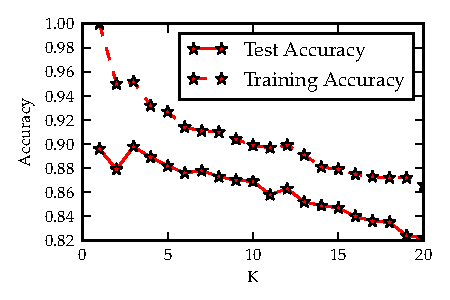
\includegraphics[width=\textwidth]{fig/multiclass/knn-accuracy}
		\caption{KNN classification accuracy on USPS.}
		\label{fig:mc-knn-acc}
	\end{subfigure}
	~
	\begin{subfigure}{.48\textwidth}
		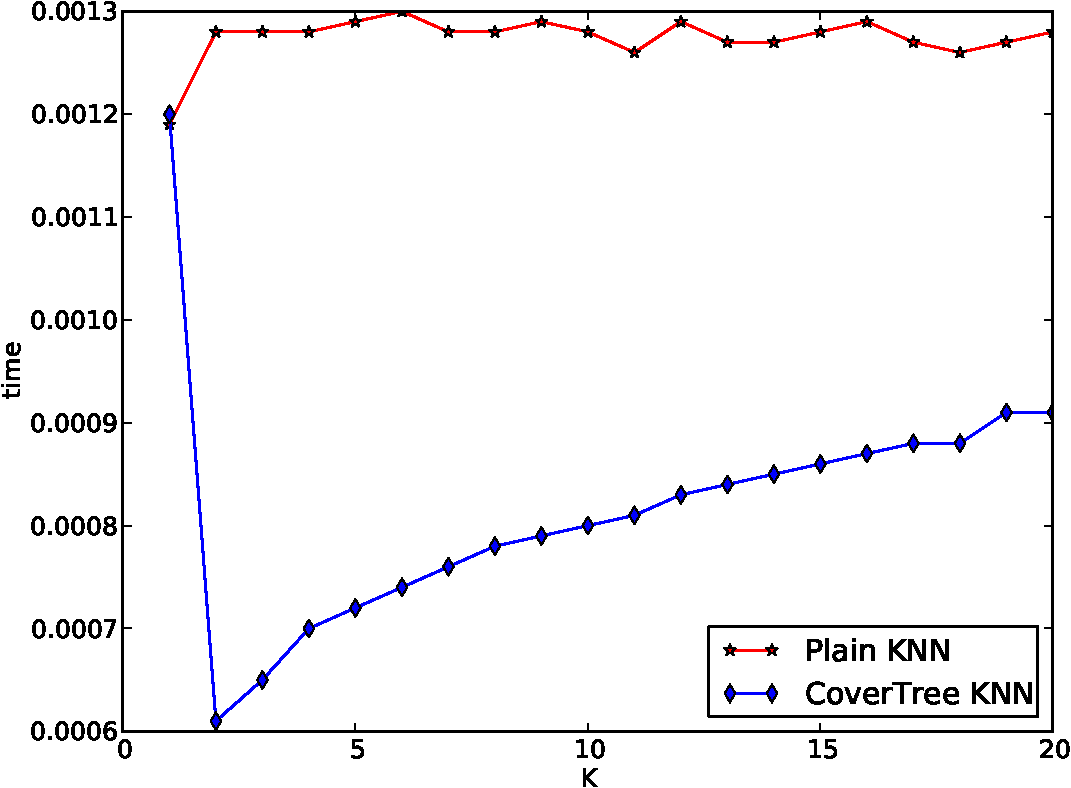
\includegraphics[width=\textwidth]{fig/multiclass/knn-time}
		\caption{Prediction time (per example) with and without CoverTree.}
		\label{fig:mc-knn-time}
	\end{subfigure}
	\caption{KNN classification on a random subset (1000 samples) of USPS.}
\end{figure}

Although simple and elegant, KNN is generally very resource costly. Because all
the training samples are to be memorized literally, the memory cost of KNN
``learning'' becomes prohibitive when the dataset is huge. Even though the
memory is big enough to hold all the data, the prediction will be slow, since
the distances between the query point and all the training points need to be
computed and ranked. The situation becomes worse if in addition the data
samples are all very high-dimensional.

\subsection{Naive Bayes}
\emph{Naive Bayes} is a simple and fast algorithm for multiclass learning.
Formally, it predict the class by computing the posterior probability of each
class $k$ after observing the input $x$:

\[
	P\left( Y=k | X = x \right) = \frac{P(X=x|Y=k)P(Y=k)}{P(X=x)}
\]

The prediction is then made by

\[
	y = \argmax_{k\in\{1,\ldots,K\}} P(Y=k|X=x)
\]

Since $P(X=x)$ is a constant factor for all $P(Y=k|X=x)$, $k=1,\ldots,K$, there
is no need to compute it.

In \shogun{}, \shogunclass{CGaussianNaiveBayes} implements the Naive Bayes
algorithm. It is prefixed with ``Gaussian'' because the probability model for
$P(X=x|Y=k)$ for each $k$ is taken to be a multi-variate Gaussian distribution.
Furthermore, each dimension of the feature vector $X$ is assumed to be
independent. The ``Naive'' independence assumption enables us the learn the
model very quickly, and is also the reason for its name. Although the
independent assumption is usually considered to be too optimistic in reality,
Naive Bayes sometimes works very well in some applications. For example, in
email spam filtering, Naive Bayes\footnote{More specifically, the discrete
	Naive Bayes is generally used in this scenario. The main difference with
	Gaussian Naive Bayes is that a tabular instead of a parametric Gaussian
	distribution is used to describe the likelihood $P(X=x|K=k)$.} is a very
popular and widely used method.

This algorithm is closely related to the \emph{Gaussian Mixture Model} (GMM) learning
algorithm. However, while GMM is an unsupervised learning algorithm, Gaussian
Naive Bayes is supervised learning. It uses the training labels to directly
estimate the Gaussian parameters for each class, thus avoids the iterative
\emph{Expectation Maximization} procedures in GMM.

\section{Reduction to Binary Problems}
\label{sec:multiclass-reduction}

Since binary classification problems are one of the most thoroughly studied
problems in machine learning, it is very appealing to consider reducing
multiclass problems to binary ones. Then many advanced learning and
optimization techniques as well as generalization bound analysis for binary
classification can be utilized.

In \shogun{}, the strategies of reducing a multiclass problem to binary
classification problems are described by an instance of
\shogunclass{CMulticlassStrategy}. A multiclass strategy describes
\begin{enumerate}
\item How to train the multiclass machine as a number of binary machines?
	\begin{itemize}
		\item How many binary machines are needed?
		\item For each binary machine, what subset of the training samples are
			used, and how are they colored\footnote{In multiclass problems, we
				use \emph{coloring} to refer partitioning the classes into two
				groups: $+1$ and $-1$, or black and white, or any other meaningful
				names.}?
	\end{itemize}
\item How to combine the prediction results of binary machines into the final
	multiclass prediction?
\end{enumerate}

The user can derive from the virtual class \shogunclass{CMulticlassStrategy} to
implement a customized multiclass strategy. But usually the built-in strategies
are enough for general problems. We will describe the built-in \emph{One-vs-Rest},
\emph{One-vs-One} and \emph{Error-Correcting Output Codes} strategies in the
following subsections.

The basic routine to use a multiclass machine with reduction to binary problems
in shogun is to create a generic multiclass machine and then assign a particular
multiclass strategy and a base binary machine.

\subsection{One-vs-Rest and One-vs-One}

The \emph{One-vs-Rest} strategy is implemented in
\shogunclass{CMulticlassOneVsRestStrategy}. As indicated by the name, this
strategy reduce a $K$-class problem to $K$ binary sub-problems. For the $k$-th
problem, where $k\in\{1,\ldots,K\}$, the samples from class $k$ are colored as
$+1$, and the samples from other classes are colored as $-1$. The multiclass
prediction is given as

\[
	f(x) = \argmax_{k\in\{1,\ldots,K\}} f_k(x)
\]
where $f_k(x)$ is the prediction of the $k$-th binary machines.

The One-vs-Rest strategy is easy to implement yet produces the good performance
in many cases. One interesting paper \citep{OneVsRestDefense} shows that the
One-vs-Rest strategy can be

\begin{quote}
	\emph{as accurate as any other approach, assuming that the underlying binary
classifiers are well-tuned regularized classifiers such as support vector
machines.}
\end{quote}

Implemented in \shogunclass{CMulticlassOneVsOneStrategy}, the 
\emph{One-vs-One} strategy \citep{OneVsOne} is another simple and intuitive 
strategy: it basically produces one binary problem for each pair of classes.  
So there will be $\binom{K}{2}$ binary problems. At prediction time, the 
output of every binary classifiers are collected to do voting for the $K$ 
classes. The class with the highest vote becomes the final prediction.

Compared with the One-vs-Rest strategy, the One-vs-One strategy is usually more
costly to train and evaluate because more binary machines are used.

In the following, we demonstrate how to use \shogun{}'s One-vs-Rest and 
One-vs-One multiclass learning strategy on the USPS dataset.  For 
demonstration, we randomly 200 samples from each class for training and 200 
samples from each class for testing.
\todo[inline]{How to organize and reference example code for tutorial?}

\begin{table}\centering
	\begin{tabular}{cccc}
	\toprule
	Strategy & Training Time & Test Time & Accuracy \\
	\midrule
	One-vs-Rest & 1.72       & 2.25      & 92.05\%  \\
	One-vs-One  & 2.14       & 4.45      & 93.75\%  \\
	\bottomrule
	\end{tabular}
	\caption{Comparison of One-vs-Rest and One-vs-One multiclass reduction
		strategy on the USPS dataset.}
	\label{tab:ovr-vs-ovo}
\end{table}

The \shogunclass{CLibLinear} is used as the base binary classifier in a
\shogunclass{CLinearMulticlassMachine}, with One-vs-Rest and One-vs-One
strategies. The running time and performance is reported in
Table~\ref{tab:ovr-vs-ovo}.

\subsection{Error-Correcting Output Codes}

\emph{Error-Correcting Output Codes} (ECOC) \citep{ECOC95,ECOCUnify} is a
generalization of the One-vs-Rest and One-vs-One strategies.

\section{Tree-style Algorithms}
\label{sec:multiclass-tree}
